\begin{figure}[htbp]

\begin{center}
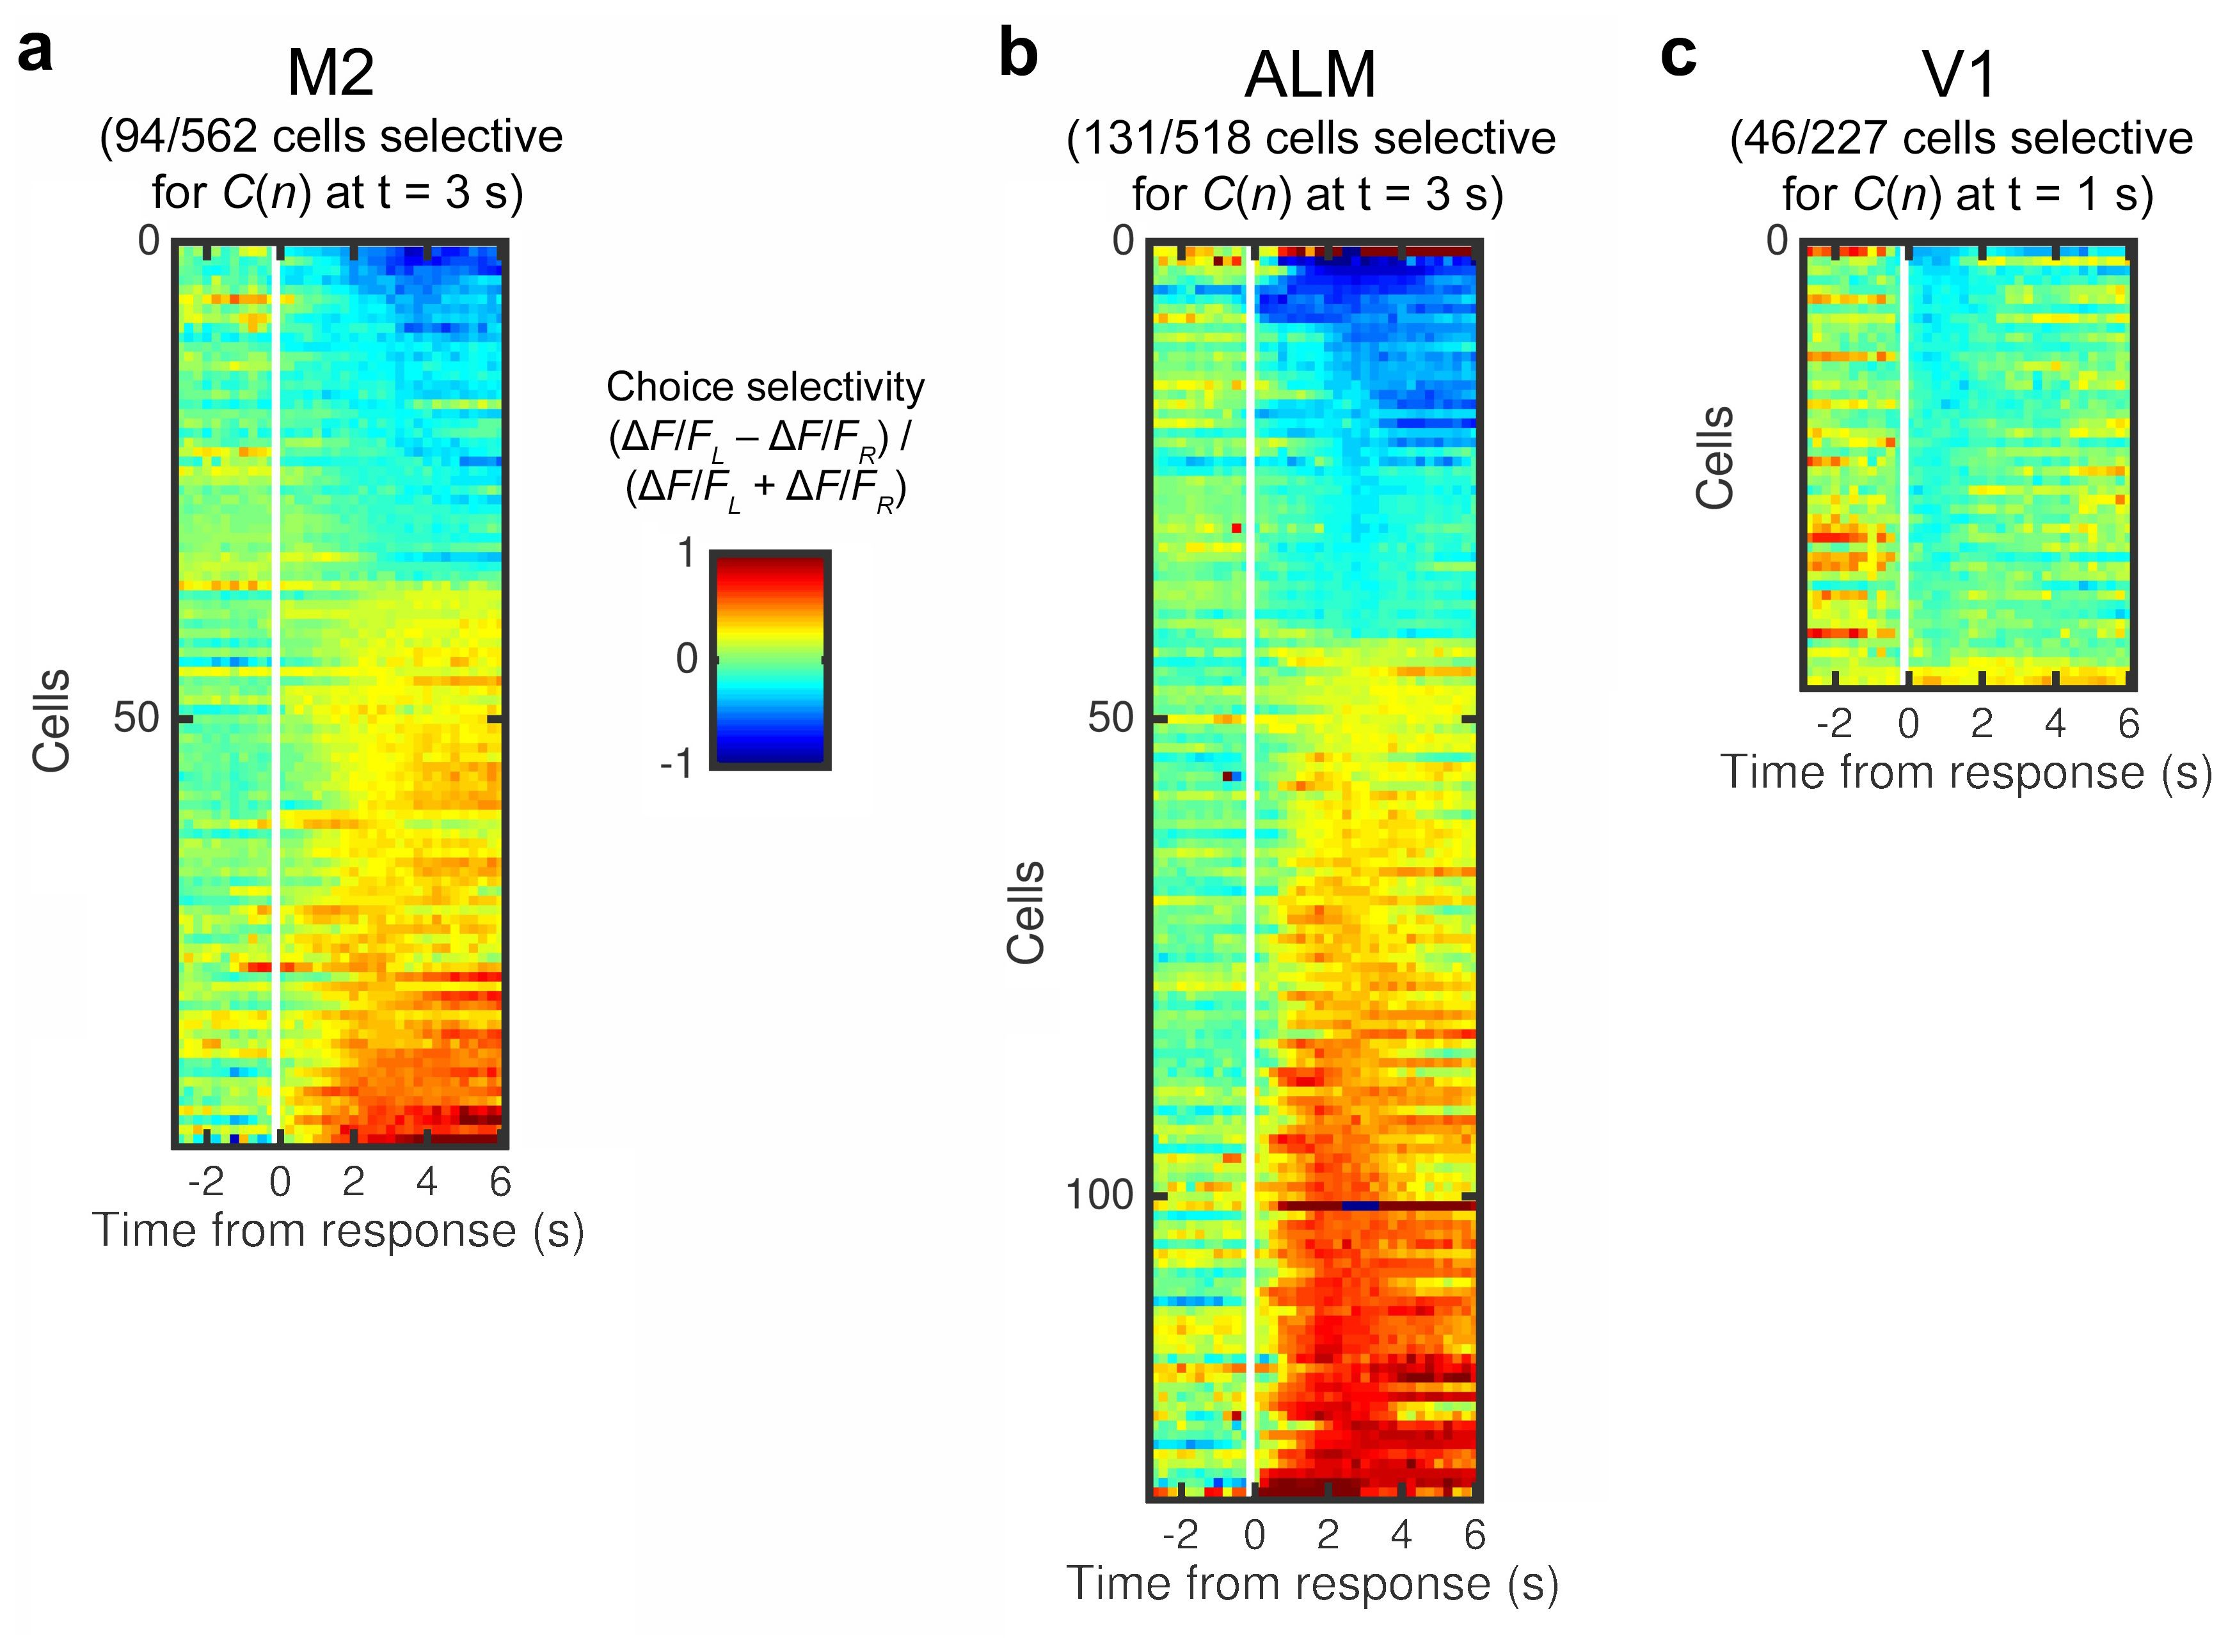
\includegraphics[width=\textwidth]{Figures/Chapter3/NN_figS8.jpg} 
\end{center}

\caption[Choice selectivity of neurons in M2, ALM, and V1]
{
Choice selectivity of neurons in M2, ALM, and V1.
(a) Selectivity for current choice was quantified by calculating the normalized $\Delta F/F$ difference during pre-switch, sound-guided trials. Each row represents an M2 neuron. Only M2 neurons that were significant for the current choice $C(n)$ at $t=3$ s from response are plotted. Cells are sorted by their choice selectivity. $N=9$ sessions from 5 mice. (b) Same as \emph{a} for ALM. $N=8$ sessions from 4 mice. (c) Same as \emph{a} for V1. Neurons that were significant for the current choice $C(n)$ at $t=1$ s from the response are plotted. $N=4$ sessions from 2 mice.
}

\label{fig:NN_figS8}
\end{figure}